%%%%%%%%%%%%%%%%%%%%%%%%%%%%%%%%%%%%%%%%%%%%%%%%%%%%%%%%%%%%%%%%%%
%%	    mmm  mmmmmm mm   m        m    m mmmmmm mmmmmm          %%
%%	  m"   " #      #"m  #        #    # #           #      	%%
%%	  #   mm #mmmmm # #m #        #    # #mmmmm     #        	%%
%%	  #    # #      #  # #  """   #    # #         #	        %%
%%	   "mmm" #mmmmm #   ##        "mmmm" #mmmmm  #          	%%
%%								                                %%
%%                                                              %%
%%                                                              %%
%%      Grundlagen der Elektrischen Netzwerke, UE               %%
%%      Gruppe 5, Team F                                        %%
%%      Authors: Severin Wolf, Maximilian Seidler.              %%
%%%%%%%%%%%%%%%%%%%%%%%%%%%%%%%%%%%%%%%%%%%%%%%%%%%%%%%%%%%%%%%%%%
\documentclass[a4paper]{article}
\usepackage{amsmath}
\usepackage[utf8]{inputenc}
\usepackage[T1]{fontenc}
\usepackage[english]{babel}
\usepackage{geometry}
\usepackage{graphicx}
\usepackage{tikz}
\usepackage{listings}
\usepackage{trfsigns}
\geometry{a4paper,left=3cm,right=2cm, top=2cm, bottom=2cm} 
\usepackage[EFvoltages, european, straightvoltages]{circuitikz}

%tikz
\ctikzset{resistor = european}
\usetikzlibrary{decorations.pathreplacing}

%no paragraph indent
\setlength{\parindent}{0pt}

%for math, that does not fit
\renewcommand*{\arraystretch}{1.3}
\newcommand\scalemath[2]{\scalebox{#1}{\mbox{\ensuremath{\displaystyle #2}}}}

\newcommand\blfootnote[1]{%
	\begingroup
	\renewcommand\thefootnote{}\footnote{#1}%
	\addtocounter{footnote}{-1}%
	\endgroup
}

% upright differenzial symbol with good spacing included!!!
\makeatletter
\providecommand*{\diff}%
	{\@ifnextchar^{\DIfF}{\DIfF^{}}}
\def\DIfF^#1{%
	\mathop{\mathrm{\mathstrut d}}%
		\nolimits^{#1}\gobblespace
}
\def\gobblespace{%
	\futurelet\diffarg\opspace}
\def\opspace{%
	\let\DiffSpace\!%
	\ifx\diffarg(%
		\let\DiffSpace\relax
	\else
		\ifx\diffarg\{%
			\let\DiffSpace\relax
		\else
			\ifx\diffarg\{%
				\let\DiffSpace\relax
			\fi\fi\fi\DiffSpace}

\begin{document}
\pagestyle{empty} \enlargethispage*{25cm}\samepage{
\vspace*{-3cm}
\begin{center}
\begin{minipage}[!h]{16cm}
\hspace*{0.2cm}

\includegraphics[width=3.3cm]{./Figures/igte_logo}
\begin{tabular}{p{8cm}}
\vspace{0.2cm}
\centering{
\Large Institute of Fundamentals and Theory in
 Electrical Engineering\\
Graz University of Technology\\
~\\}
\end{tabular}

\includegraphics[width=3.3cm]{./Figures/TUG_logo}
\end{minipage}
	\Large
	\textbf{Fundamentals of Electrical Circuits} \vspace*{0.5cm}\\
	\textbf{Homework 7}\\
	Laplace-Transformation
	\vspace*{0.5cm}
	
	\large
	6 May 2021
	\end{center}}

	\vspace*{1cm}
	
	%%%%%%%%%%%%%%%%%%%%%%%%%%%%%%%%%%%%%%%%%%%%%%%%%%%%%%%%%%%%%%%%%%%%
	%%%%%%%%%%%%%%%%%%%%%%%%%%%%%%%%%%%%%%%%%%%%%%%%%%%%%%%%%%%%%%%%%%%%
	Apply the Laplace-Transform in order to analyse the given circuit.
	\begin{enumerate}
		\item Apply the Laplace-Transform in oder to compute $U(s) = \mathcal{L}\{u(t)\}$ in the s-domain. \\
		$u(t)$ is defined by the diagram in figure \ref{fig:input}. \textbf{(0.5 Points)}
		
		\item Derive the s-domain equivalent circuit and include the possibility of inital values. \textbf{Mark the current through the capacitor in the s-domain cirucit.} Pay attention to the arrow's direction. \textbf{(0.5 Points)}
		
		\item Derive the expression for the voltage across the capacitor $U_C(s)$ in the s-domain by applying KCL and KVL to the circuit. The initial condition for the capacitor is given as $u_C(t=0) = 0\,\text{V}$ and can be used to simplify the equations. \textbf{(1 Point)}

		\item Find the time-domain expressions for the voltage $u_C(t) = \mathcal{L}^{-1}\{U_C(s)\}$ for the given input signal. Calculate the time constant $\tau$ for this first order circuit. \textbf{(1.5 Points)}

		\item Plot the voltage $u_C(t)$ across the capacitor for $0 \leq t \leq 4T$ in \textsc{Matlab}. \textbf{(0.5 Points)}
		
		\item Simulate the circuit in LTSpice for the given input voltage $u(t)$ for the same time-intervall and compare the results. \textbf{(1 Point)}
	\end{enumerate}
		

	\subsection*{Values:}
	$R_1 = 100~\Omega$ \qquad $R_2 = 100~\Omega$ \qquad $R_3 = 300~\Omega$ \qquad $C=25~\mu\text{F}$ \qquad $U_0 = 2.5~\text{V}$ \qquad $T = 4~\text{ms}$\\
	
	\begin{figure}[!htb]
		\begin{minipage}{0.4\textwidth}
			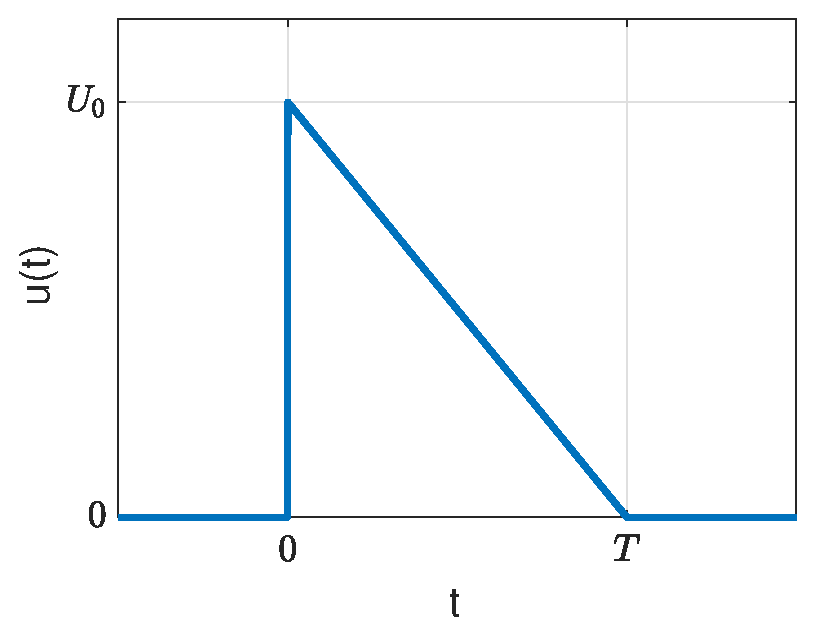
\includegraphics[width=1\textwidth]{./Figures/input-signal.eps}
			\caption{Input-Signal}
			\label{fig:input}
		\end{minipage}\hfill
		\begin{minipage}{0.4\textwidth}
			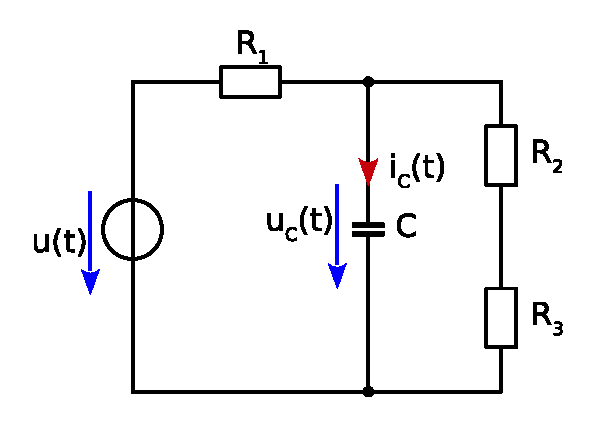
\includegraphics[width=1\textwidth]{./Figures/homework7_circuit.eps}
			\caption{Circuit}
			\label{fig:circuit}
			\vspace{1cm}
		\end{minipage}
	\end{figure}
	
	
	\blfootnote{Deadline: 13 May 2021; Presentation: Team 7 \\
		presentation: 14 May 2021 at 9o'Clock (attendence is voluntary!) \\
	Link to the presentation-meeting: https://tugraz.webex.com/tugraz/j.php?MTID=ma0812eff6637ffbf004e8bab03ee5f70}

\newpage
\section{Solution}
\subsection{Lapalce-Transformation of $u(t)$}
As $u(t)$ is given as a diagram, we first have to determine the function $u(t)$. Therefore we devide $u(t)$ into three parts, which we will add up.
\begin{align*}
	u_1(t) = U_0 \cdot \sigma(t) \;\;\; &\laplace \;\;\; U_1(s) = U_0 \cdot \frac{1}{s}\\
	u_2(t) = -\frac{U_0}{T}t \cdot \sigma(t) \;\;\; &\laplace \;\;\; U_2(s) = -\frac{U_0}{T} \cdot \frac{1}{s^2}\\
	u_3(t) = \left(\frac{U_0}{T}t-U_0 \right) \cdot \sigma\left(t-T\right) \;\;\; &\laplace \;\;\; 
	U_3(s) = \frac{U_0}{T} \cdot \frac{1}{s^2} \cdot e^{-Ts}\\
	u(t) = U_0 \cdot \sigma(t) - \frac{U_0}{T}t \cdot \sigma(t) + \left(\frac{U_0}{T}t-U_0 \right) \cdot \sigma\left(t-T \right) \;\;\; &\laplace \;\;\;
	U(s) = U_0 \cdot \frac{1}{s} - \frac{U_0}{T} \cdot \frac{1}{s^2} + \frac{U_0}{T} \cdot \frac{1}{s^2} \cdot e^{-Ts}\\
	U(s) = 2.5 \cdot \frac{1}{s} - 625 \cdot \frac{1}{s^2} + 625 \cdot \frac{1}{s^2} \cdot e^{-0.004s}\\
\end{align*}

\subsection{Transformation of the Network}
In order to find $U_C(s)$ we have to transform the Network into the s-domain.
\begin{figure}[!h]\centering
	\begin{circuitikz}[scale=0.75, transform shape]
		\draw(0,0)
		to[short](0,1)
		to[V, v=$U(s)$,](0,4)
		to[short](0,5) to[short](1,5)
		to[R, l=$R_1$](4,5)
		to[short, -*](5,5)
		to[short, -*, i=$I_C(s)$, color=red](5,4.5)
		to[short](7,4.5) to[short, i=$sCU_C(s)$, color=red](7,3)
		to[C, l=$\frac{1}{sC}$, v=$U_c(s)$](7,2)
		to[short](7,0.5) to[short](5,0.5) to[short](5,0)
		to[short](0,0);
		\draw(5,4.5)
		to[short, *-](3,4.5) to[short, i<=$CU_C(0)$, color=red](3,3)
		to[I](3,2)
		to[short](3,0.5) to[short, -*](5,0.5);
		\draw(5,5)
		to[short](9,5) to[short](9,4.5)
		to[R, l=$R_2$](9,2.5)
		to[R, l=$R_3$](9,0.5)
		to[short](9,0) to[short](5,0);
	\end{circuitikz}	
\end{figure}

\subsection{Determination of $U_C(s)$}
\begin{align*}
	U_C(s) = U(s) \cdot \frac{\frac{\frac{1}{sc}\cdot (R_2+R_3)}{\frac{1}{sc} + (R_2+R_3)}}{R_1 + \frac{\frac{1}{sc}\cdot (R_2+R_3)}{\frac{1}{sc} + (R_2+R_3)}}\\
	U_C(s) = \left(2.5 \cdot \frac{1}{s} - 625 \cdot \frac{1}{s^2} + 625 \cdot \frac{1}{s^2} \cdot e^{-0.004s} \right) \cdot \frac{\frac{\frac{1}{25\cdot10^{-6}\cdot s}\cdot (100+300)}{\frac{1}{25\cdot10^{-6}\cdot s} + (100+300)}}
	{100 + \frac{\frac{1}{25\cdot10^{-6}\cdot s}\cdot (100+300)}{\frac{1}{25\cdot10^{-6}\cdot s} + (100+300)}} =
	U(s) \cdot \frac{400}{s+500}\\
\end{align*}

\subsection{Inverse Laplace, back to time domain}

\begin{align*}
	2,5\cdot\frac{1}{s^2} &\Laplace \;\;\; 2,5\cdot t\\
	625\cdot \frac{1}{s^3} \;\;\; &\Laplace \;\;\; 625\cdot \frac{t^2}{2}\\
	625\cdot \frac{1}{s^3} \cdot e^{-2,5s}\;\;\; &\Laplace \;\;\; 
	(t-2.5)\\
	u(t) = U_0 \cdot \sigma(t) - \frac{U_0}{T}t \cdot \sigma(t) + \left(\frac{U_0}{T}t-U_0 \right) \cdot \sigma\left(\frac{U_0}{T}t-U_0 \right) \;\;\; &\laplace \;\;\;
	U(s) = U_0 \cdot \frac{1}{s} - \frac{U_0}{T} \cdot \frac{1}{s^2} + \frac{U_0}{T} \cdot \frac{1}{s^2} \cdot e^{-U_0s}\\
	U(s) = 2.5 \cdot \frac{1}{s} - 625 \cdot \frac{1}{s^2} + 625 \cdot \frac{1}{s^2} \cdot e^{-2.5s}\\
\end{align*}


\end{document}
